% Source: Code/vrifa/presentation.tex

\documentclass[border=4pt]{standalone}
\usepackage{graphicx}
\usepackage{tikz}
\usepackage{xcolor}
\usetikzlibrary{shapes.geometric, arrows.meta, positioning, fit, calc}

\definecolor{garnet}{HTML}{73000a}
\definecolor{darkgarnet}{HTML}{570008}
\definecolor{atlantic}{HTML}{466A9F}
\definecolor{congaree}{HTML}{1F414D}
\definecolor{horseshoe}{HTML}{65780B}
\definecolor{honeycomb}{HTML}{A49137}
\definecolor{gray90}{HTML}{363636}
\definecolor{gray70}{HTML}{5C5C5C}
\definecolor{gray50}{HTML}{A2A2A2}

\begin{document}
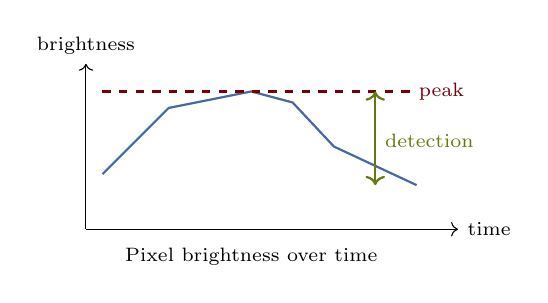
\begin{tikzpicture}[scale=0.7, xscale=1.5]
    \draw[->] (0,0) -- (4.5,0) node[right, scale=1, transform shape=false] {\scriptsize time};
    \draw[->] (0,0) -- (0,3) node[above, scale=1, transform shape=false] {\scriptsize brightness};

    % Brightness curve
    \draw[thick, atlantic] (0.2,1) -- (1,2.2) -- (2,2.5) -- (2.5,2.3) -- (3,1.5) -- (4,0.8);

    % Peak line
    \draw[dashed, garnet, thick] (0.2,2.5) -- (4,2.5);
    \node[garnet, font=\scriptsize, scale=1, transform shape=false] at (4.3,2.5) {peak};

    % Detection zone
    \draw[<->, horseshoe, thick] (3.5,0.8) -- (3.5,2.5);
    \node[horseshoe, font=\scriptsize, right, scale=1, transform shape=false] at (3.5,1.6) {detection};

    \node[font=\scriptsize, scale=1, transform shape=false] at (2,-0.5) {Pixel brightness over time};
\end{tikzpicture}
\end{document}
